\chapterA{Hito 4 - Prototipado en Papel}

La siguiente fase del Diseño Guiado por Objetivos (DGO) que vamos a abordar es el prototipado. Esta etapa se va a dividir en dos etapas claramente diferenciadas:
el prototipado en papel (este hito) y el prototipado digital (siguiente hito). Para realizar este prototipado en papel se ha definido un proceso dividido en seis
etapas (con posibilidad de realizar una segunda iteración). \\

En estas etapas se va a definir tanto la estructura de alto nivel y la organización de las pantallas como el flujo, comportamiento y organización del sistema. Estas
etapas son las siguientes y se han realizado de acuerdo al orden que aparecen descritas a continuación:
\begin{enumerate}
    \item \textbf{Definir el factor de forma, la postura y los métodos de entrada}
    \item \textbf{Definir los elementos de datos y funcionales}
    \item \textbf{Determinar los grupos funcionales y las jerarquías}
    \item \textbf{Construir los escenarios key path}
    \item \textbf{Hacer un prototipo del framework de interacción}
    \item \textbf{Validar los diseños con los escenarios de validación}
\end{enumerate}
% TODO argumentar el orden de las etapas 3, 4 y 5.
% TODO introducir los dos siguientes apartados (resultados Hito 3)

\section{Escenarios de contexto}
Un escenario es una situación narrativa, una historia concreta y realista que involucra a una persona y narra de manera detallada cómo persigue un objetivo y
finalmente logra satisfacer dicho objetivo, describiendo el proceso que ha seguido para ello. Cada uno de estos escenarios va a describir cómo se va a comportar
el usuario (en este caso la persona) en el contexto de la aplicación, definiendo en todo momento qué es lo que tiene que realizar para poder afrontar un problema
concreto.
\subsection{Escenarios de contexto de Marta}
\begin{itemize}
    \item \textbf{Gira detallada por Italia} $\rightarrow$ Hace unos días Francesca anunció una gira por el norte de Italia, donde Marta todavía no había estado. 
    Marta y su hermano no se pueden perder esto, por lo que saca la aplicación y selecciona como destino Nápoles, donde Francesca dará su primer concierto. 
    Al buscar esta ciudad como destino, aparecen listados por ordenados por horarios (por defecto, pero con posibilidad de cambiarlo) las distintas opciones 
    que se ofrecen para viajar allí desde Madrid. Como no han visitado estas ciudades van a necesitar informarse bien para hacer la ruta de modo que lleguen 
    a tiempo al concierto y puedan hacer algo de turismo antes de ponerse en marcha al siguiente destino del tour, para ello han estudiado tanto ella como su hermano 
    bien los tipos de transporte, horarios y servicios que ofrecen estos y más información adicional (como las compañías, estaciones, paradas, etc.) 
    que han podido consultar en la aplicación sin tener que salirse de esta. En algunas ciudades no encontraron alojamiento por lo que van a tener 
    que recurrir a medios de transporte que ofrezcan camas y necesitarán, por lo tanto, seleccionar este servicio. \\ 

    Tras haber barajado todas las opciones posibles de las que ofrecía la aplicación, finalmente se decidieron por el primer vuelo con destino a Nápoles 
    que salía de Madrid, de modo que podrían aprovechar la mañana para instalarse en el motel y hacer un poco de turismo por la ciudad. Por ello finalmente 
    compran los billetes en la app y luego pueden consultarlos en su perfil.
    
    \item \textbf{Cambio de planes por motivo económico} $\rightarrow$ Es época de exámenes y Marta está muy agobiada. No está muy segura de si ha aprobado 
    las asignaturas que lleva o de cómo le van a salir las que le faltan. Su amiga Pili, viendo el agobio de Marta, le ha dicho de irse a Ibiza de fiesta 
    el finde posterior a los exámenes, de esta manera tiene mayor aliciente para continuar con las semanas que le quedan. A Marta le encantó la idea, así 
    que enseguida sacó la app y buscó vuelos ese finde a Ibiza. Desgraciadamente, estaba un poco justa de dinero porque no está trabajando por el momento, 
    y los precios que tenía el vuelo eran demasiado caros para su bolsillo. Afortunadamente, pudo ver en la aplicación que el mismo día salía un vuelo a 
    Palma de Mallorca, y les costaba la ida y vuelta 50€ menos y seleccionaron esta opción junto con los asientos que les parecían más adecuados para estar 
    juntas. Al final a Pili le pareció bien cambiar el plan de fiesta a un plan de playa, así que compraron los billetes, deseosas de que acaben.
\end{itemize}
\subsection{Escenarios de contexto de Isabel}
\begin{itemize}
    \item \textbf{Viaje inesperado} $\rightarrow$ Es lunes e Isabel va a tomar un café con sus compañeros de trabajo, como de costumbre. Mientras espera 
    a que le traigan el desayuno, su móvil empieza a sonar y al mirar quién la está llamando, ve que es su jefe. Éste le dice que el miércoles hay una 
    conferencia para la inclusión de niños con discapacidad y que la mujer que iba a dar la ponencia ha tenido un imprevisto y no podrá darla, por 
    lo que le ofrece a Isabel sustituirla. \\

    Aunque es muy precipitado, Isabel acepta y empieza a buscar transporte. Abre la aplicación y selecciona en el apartado filtros, persona 
    con discapacidad física, y ve el abanico de posibilidades de vuelos accesibles para ella y la información detallada que ofrecen para asegurarse 
    que efectivamente es accesible para gente con discapacidad física que requieran de silla de ruedas. Al ser un viaje que no tenía previsto, su objetivo 
    es ahorrar el máximo dinero posible, por lo escoge el más barato. Contenta con su compra, se va a casa a preparar la maleta.
    \item \textbf{Problemas con la compra} $\rightarrow$ Carmen e Isabel llevan varios meses intentando ir a la exposición de arte de un artista emergente 
    que les gusta mucho. En Barcelona las entradas se agotaron a los pocos minutos de salir, por lo que no consiguieron. Ahora ha vuelto con otra exposición, 
    pero esta vez en Madrid. \\

    Como Carmen e Isabel no se la quieren perder, han decidido que viajarán a Madrid un par de días. La exposición estará un mes entero, pero no saben qué días irán.
    Isabel abre la aplicación y busca los trenes de Renfe en el mes completo que más se ajustan a sus horarios. Eligen esta compañía ya que Carmen tiene descuentos. 
    Cuando ya ha comprado los billetes, espera un período de tiempo para recibirlos en su correo, pero no llegan. Desde la aplicación se pone en contacto con el 
    servicio al cliente, que le dice que están teniendo problemas con la gestión de los billetes y que se lo resuelven de forma manual en pocos minutos. Y así fue, 
    instantes después, Isabel ya tenía sus billetes.
\end{itemize}

\section{Requisitos}
Tras hacer un estudio de problemas, expectativas y escenarios de contexto, la última etapa de esta fase de requisitos. En esta fase se van a exponer claramente las 
necesidades de la persona para satisfacer sus objetivos. Dicho de otro modo, se trata de definir qué es lo que va a hacer nuestra aplicación (pero sin entrar en
detalle en cómo lo va a hacer). Los requisitos que hemos identificado son los siguientes:
\begin{itemize}
    \item Buscar (\textit{acción}) transportes disponibles (\textit{objeto}) a las ciudades designadas (\textit{contexto}).
    \item Seleccionar (\textit{acción}) fechas concretas o un intervalo de tiempo(\textit{objeto}) para la búsqueda del transporte (\textit{contexto}).
    \item Comparar (\textit{acción}) precios (\textit{objeto}) de los diferentes transportes a la ciudad designada (\textit{contexto}).
    \item Reservar (\textit{acción}) billetes (\textit{objeto}) de los transportes deseados (\textit{contexto}).
    \item Ofrecer (\textit{acción}) información sobre horarios de transporte (\textit{objeto}) al realizar la búsqueda (\textit{contexto}).
    \item Ofrecer (\textit{acción}) información de los asientos disponibles (\textit{objeto}) del vehículo seleccionado (\textit{contexto}).
    \item Seleccionar (\textit{acción}) asientos (\textit{objeto}) una vez elegido el transporte (\textit{contexto}).
    \item Ofrecer (\textit{acción}) diferentes rutas (\textit{objeto}) cuando seleccionas una serie de destinos (\textit{contexto}).
    \item Ofrecer (\textit{acción}) servicios disponibles en el transporte (\textit{objeto}) cuando seleccionas un transporte en concreto (\textit{contexto}).
    \item Indicar (\textit{acción}) la zona de recogida, origen y destino (\textit{objeto}) del vehículo a lo largo del trayecto (\textit{contexto}).
    \item Filtrar (\textit{acción}) opciones de transporte (\textit{objeto}) específicas para personas con discapacidad física (\textit{contexto}).
    \item Mostrar (\textit{acción}) información detallada (\textit{objeto}) sobre la accesibilidad de los transportes disponibles (\textit{contexto}).
    \item Ofrecer (\textit{acción}) soporte al cliente (\textit{objeto}) para resolver problemas de gestión de billetes de manera rápida y eficaz (\textit{contexto}).
    \item Realizar (\textit{acción}) reservas (\textit{objeto}) para un número determinado de personas (\textit{contexto}).
    \item Filtrar (\textit{acción}) viajes (\textit{objeto}) en función del número de personas que vayan a participar en el viaje (\textit{contexto}).
    \item Reservar (\textit{acción}) conjuntos de asientos (\textit{objeto}) para que todos los viajeros en caso de que sea un grupo puedan sentarse juntos (\textit{contexto}).
    \item Notificar al usuario (\textit{acción}) que la reserva (\textit{objeto}) se ha realizado correctamente (\textit{contexto}).
    \item Poder consultar (\textit{acción}) una reserva (\textit{objeto}) cuando el usuario lo desee (\textit{contexto})
    \item Poder cancelar (\textit{acción}) una reserva (\textit{objeto}) en caso de que el usuario lo considere pertinente (\textit{contexto}).
    \item Poder modificar (\textit{acción}) una reserva (\textit{objeto}) en caso de que el usuario lo considere pertinente (\textit{contexto}).
    \item Elegir (\textit{acción}) la ruta (\textit{objeto}) que más se ajuste a tus necesidades en caso de que haya varias opciones que se puedan seleccionar (\textit{contexto}).
    \item Consultar (\textit{acción}) las paradas (\textit{objeto}) de una ruta en caso de que las tenga (\textit{contexto}).
    \item Ofrecer (\textit{acción}) opciones de hacer escalas (\textit{objeto}) en caso de que se quiera hacer un vuelo con estas condiciones (\textit{contexto}).
    \item Filtrar (\textit{acción}) tipo de transporte (\textit{objeto}) según el precio (\textit{contexto}).
    \item Filtrar (\textit{acción}) tipo de transporte (\textit{objeto}) según los horarios (\textit{contexto}).
    \item Filtrar (\textit{acción}) tipo de transporte (\textit{objeto}) según el origen y el destino (\textit{contexto}).
    \item Ordenar (\textit{acción}) los transportes (\textit{objeto}) por precio según las necesidades, para agilizar la búsqueda (\textit{contexto}).
    \item Ordenar (\textit{acción}) los transportes (\textit{objeto}) por horarios según las necesidades, para agilizar la búsqueda (\textit{contexto}).
\end{itemize}

\section{Factor de forma, postura y métodos de entrada}
% TODO Introducción del apartado
\subsection{Factor de forma}
Nuestra aplicación estará diseñada para móvil y ordenador. Si se utiliza desde el ordenador, la aplicación se utilizará en mayoritariamente en casa para 
poder organizar el viaje  tranquilamente, aunque también puede utilizarse en un contexto de trabajo en el que el usuario esté en una oficina. Si se utiliza 
la aplicación desde el móvil, normalmente el contexto cambia mucho, y el usuario hará un uso de la aplicación rápido y de consulta de información y puede 
realizarse en cualquier parte y momento.

\subsection{Postura}
Por un lado tenemos varias \underline{posturas soberanas} centradas en toda la parte de buscar destino, comparación de precios, ofertas o destinos a los que acudir 
según las preferencias indicadas por el usuario. Por otro lado tendríamos una \underline{postura temporal} relacionada con el chat de soporte o con diferentes dudas 
que le puedan surgir al usuario que necesiten ser subsanadas, así como diferentes reseñas que los usuarios hayan escrito sobre los diferentes destinos. Por último 
tendríamos una \underline{postura demonio} relacionada con las diferentes notificaciones que puedan surgir mediante el uso de la aplicación (como la calificación o 
respuesta a una reseña hecha) y las preferencias indicadas por el usuario.

\subsection{Métodos de entrada}
En caso de que se utilice la aplicación vía ordenador, los métodos de entrada serán el teclado y ratón, mientras que si se accede a la aplicación por el móvil, 
el método de entrada será la propia pantalla del teléfono.

\section{Elementos de datos y funcionales}
% TODO Introducción del apartado
\subsection{Elementos de datos}
\begin{itemize}
    \item \textbf{Transportes} $\rightarrow$ Medio por el cuál se va a viajar.
    \begin{itemize}
        \item \textit{Atributos} $\rightarrow$ Horario, origen, destino, accesibilidad, tipo.
        \item \textit{Relación} $\rightarrow$ Un transporte tiene asociados tantos billetes como plazas tenga, y un transporte puede ser asociado a una ruta.
    \end{itemize}
    \item \textbf{Billetes} $\rightarrow$ Es el elemento que se paga para tener acceso al transporte.
    \begin{itemize}
        \item \textit{Atributos} $\rightarrow$ Precio, asiento, descuentos.
        \item \textit{Relación} $\rightarrow$ El billete va asociado a un transporte.
    \end{itemize}
    \item \textbf{Viajes} $\rightarrow$ Conjunto de transportes para llegar de un punto a otro.
    \begin{itemize}
        \item \textit{Atributos} $\rightarrow$ Origen, destino, transporte.
        \item \textit{Relación} $\rightarrow$ Transportes con los que se pueden hacer las rutas.
    \end{itemize}
\end{itemize} 

\subsection{Elementos funcionales}
\begin{itemize}
    \item \textbf{Buscar (acción) transportes disponibles (objeto) a las ciudades designadas (contexto)} $\rightarrow$ Desde el menú principal podemos seleccionar 
    origen, destino y fechas en las que se quiera realizar el viaje.
    \item \textbf{Filtrar (acción) opciones de transporte (objeto) específicas para personas con discapacidad física (contexto)} $\rightarrow$ Desde la pantalla 
    de comparador de viajes se pueden filtrar todas las opciones de transporte adecuadas para personas con discapacidad física
    \item \textbf{Reservar (acción) billetes (objeto) de los transportes deseados (contexto)} $\rightarrow$ Desde la pantalla de comparador de viajes se pueden 
    seleccionar los billetes deseados y reservarlos.
    \item \textbf{Mostrar (acción) información detallada sobre la accesibilidad de los transportes disponibles (objeto)} $\rightarrow$ Dentro de la información de 
    cada transporte, se puede visualizar el nivel de accesibilidad del medio de transporte y seleccionar la ayuda si el usuario lo desea.
    \item \textbf{Seleccionar (acción) asientos(objeto) una vez elegido el transporte (contexto)} $\rightarrow$ Desde la pantalla de reserva de billetes se 
    pueden seleccionar los asientos deseados.
    \item \textbf{Indicar (acción) la zona de recogida, origen y destino (objeto) del vehículo a lo largo del trayecto (contexto)} $\rightarrow$ Desde la pantalla 
    de reserva de transporte se puede visualizar los detalles de la reserva del transporte, como la recogida origen y el destino de devolución.
    \item \textbf{Ofrecer (acción) soporte al cliente (acción) para resolver problemas de gestión de billetes de manera rápida y eficaz (contexto)} $\rightarrow$ Desde 
    cualquier pantalla se puede acceder a la pantalla de atención al cliente.
    \item \textbf{Seleccionar (acción) fechas concretas o un intervalo de tiempo(objeto) para la búsqueda del transporte (contexto)} $\rightarrow$ Desde el menú 
    principal podemos seleccionar las fechas en las que se quiera realizar el viaje con un abanico de días par ofrecer flexibilidad.
    \item \textbf{Comparar (acción) precios (objeto) de los diferentes transportes a la ciudad designada (contexto)} $\rightarrow$ Desde la pantalla de comparador 
    de viajes se puede visualizar todas las opciones de transporte a la ciudad destino.
    \item \textbf{Ordenar (acción) los transportes por precios y/o fechas (objeto) según las necesidades, para agilizar la búsqueda (contexto)} $\rightarrow$ Desde 
    la pantalla de comparador de viajes se pueden ordenar los transportes por fechas y precios.
    \item \textbf{Seleccionar (acción) tipo de transporte (objeto) según preferencias y/o precio (contexto)} $\rightarrow$ Desde el menú principal podemos seleccionar 
    el vehículo concreto en el que queremos realizar el viaje.
    \item \textbf{Ofrecer (acción) información sobre horarios de transporte (objeto) al realizar la búsqueda (contexto)} $\rightarrow$ Dentro de la pagina de búsqueda 
    de viajes, aparecen los horarios disponibles para cada opción de viaje.
    \item \textbf{Ofrecer (acción) información de los asientos disponibles (objeto) del vehículo seleccionado (contexto)} $\rightarrow$ Dentro de la página de reserva 
    de transporte se puede ver cuántos asientos quedan disponibles y cuáles.
    \item \textbf{Ofrecer (acción) servicios disponibles en el transporte (objeto) cuando seleccionas un transporte en concreto (contexto)} $\rightarrow$ Dentro de la 
    página de reserva de transporte se puede ver los servicios adicionales del transporte y reservarlos.
    \item \textbf{Realizar (acción) reservas (objeto) para un número determinado de personas (contexto)} $\rightarrow$ Dentro de la página de reserva de transporte 
    se pueden seleccionar cuantos billetes se quieren comprar, distinguiendo entre adultos, niños y personas con discapacidad.
    \item \textbf{Filtrar (acción) viajes (objeto) en función del número de personas que vayan a participar en el viaje (contexto)} $\rightarrow$ Dentro de la página 
    de búsqueda de transporte, se pueden filtrar las opciones de viaje a base del número de personas que participen en el viaje.
    \item \textbf{Reservar (acción) conjuntos de asientos (objeto) para que todos los viajeros en caso de que sea un grupo puedan sentarse juntos (contexto)} 
    $\rightarrow$ Dentro de la página de reserva en el apartado de selección de asiento se pueden seleccionar los asientos deseados.
    \item \textbf{Notificar al usuario (acción) que la reserva (objeto) se ha realizado correctamente (contexto)} $\rightarrow$ Después de completar la reserva, 
    se abre una página de confirmación de reserva.
    \item \textbf{Poder consultar (acción) una reserva (objeto) cuando el usuario lo desee (contexto)} $\rightarrow$ En la página de viajes reservados, se pueden
    consultar todas las reservas realizadas.
    \item \textbf{Poder cancelar (acción) una reserva (objeto) en caso de que el usuario lo considere pertinente (contexto)} $\rightarrow$ En la página de viajes 
    reservados, se puede cancelar una reserva.
    \item \textbf{Poder modificar (acción) una reserva (objeto) en caso de que el usuario lo considere pertinente (contexto)} $\rightarrow$ En la página de viajes 
    reservados, se puede modificar una reserva.
    \item \textbf{Elegir (acción) la ruta (objeto) que más se ajuste a tus necesidades en caso de que haya varias opciones que se puedan seleccionar (contexto)}
    $\rightarrow$ Dentro de la página de comparador de viajes se puede seleccionar la ruta que se desea.
    \item \textbf{Consultar (acción) las paradas (objeto) de una ruta en caso de que las tenga (contexto)} $\rightarrow$ Dentro de la página de comparador de viajes 
    se puede consultar en cada ruta mostrada las paradas que tiene la ruta.
    \item \textbf{Ofrecer (acción) opciones de hacer escalas (objeto) en caso de que se quiera hacer un vuelo con estas condiciones (contexto)} $\rightarrow$ Dentro 
    de la página de comparador de viajes se puede seleccionar la opción de coger vuelos con escalas.
    \item \textbf{Filtrar(acción) tipo de transporte (objeto) según el precio (contexto)} $\rightarrow$ Dentro de la página de comparador de viajes se puede filtrar 
    por precio y tipo de transporte.
    \item \textbf{Seleccionar (acción) tipo de transporte (objeto) según los horarios (contexto)} Dentro de la pagina de busqueda de transporte, se puede seleccionar 
    una opción de transporte en un horario específico.
    \item \textbf{Ordenar (acción) los transportes (objeto) por precio según las necesidades, para agilizar la búsqueda (contexto)} $\rightarrow$ Dentro de la página 
    de búsqueda, se pueden ordenar las opciones por precio (mayor a menor / menor a mayor).
    \item \textbf{Ordenar (acción) los transportes (objeto) por horarios según las necesidades, para agilizar la búsqueda (contexto)} $\rightarrow$ Dentro de la página 
    de búsqueda, se pueden ordenar las opciones por horarios.
    \item \textbf{Ordenar (acción) los transportes (objeto) por duración de trayecto, para agilizar la búsqueda (contexto)} $\rightarrow$ Dentro de la página de 
    búsqueda, se pueden ordenar las opciones por duración de trayecto (menor a mayor).
\end{itemize}

\section{Grupos funcionales y jerarquías}
% TODO Introducción del apartado

\begin{figure}[H]
    \centering
    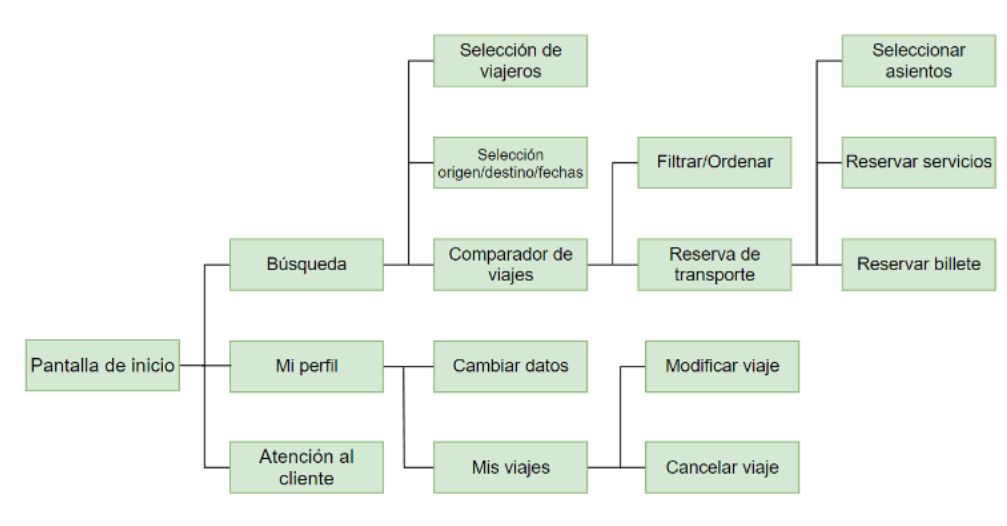
\includegraphics[width=0.8\linewidth]{./Imagenes/jerarquia.png}
    \caption{Diagrama de jerarquías de funciones}
    \label{fig:jerarquias}
\end{figure}

\begin{itemize}
    \item La pantalla de inicio contiene los elementos de búsqueda, atención al cliente y mi perfil.
    \item El elemento de búsqueda es el componente principal por lo que ocupa gran espacio en la interfaz. Al usarla podrás realizar la selección de origen destino y/o fechas, así como de los viajeros. Estas opciones sirven como filtro a la hora de realizar la comparación, que se muestra a continuación.
    \item En el apartado de Comparador de viajes puedes ver todos los que cumplen los criterios anteriormente mencionados. Además puedes cambiar los filtros anteriores y/u ordenarlos según distintos criterios. Además podrás seleccionar si quieres que se muestren solo los viajes accesibles para personas con discapacidad física.
    \item Una vez te interesas por un viaje, pasarás al apartado de Reserva de transporte. Aquí se mostrarán todos los datos de manera clara, como se marcó en los requisitos, además de poder elegir los asientos y realizar la propia reserva del billete.
    \item En el apartado Mi perfil se puede cambiar los datos del usuario (nombre, correo, teléfono, etc) además de poder ver las reservas pasadas, pudiendo tanto cancelar el viaje como modificarlo (fecha u hora, siempre que lo permita la compañía).
    \item Como se comentó en el apartado anterior, se podrá acceder al apartado de atención al cliente desde cualquier punto de la aplicación.
    \item Un principio que podría ser útil para la aplicación es la programación orientada a objetos, debido a que tenemos distintas partes que podrían ser encapsuladas en éstos, como son los viajes.
    \item En cuanto a los patrones, uno de lo que podría usarse sería el patrón Singleton ya que asegura que cada clase tenga una única instancia, controla el acceso a cada recurso y tiene un control estricto de las variables disponibles.
    
\end{itemize}

\section{Escenarios key path}
% TODO Introducción del apartado

\subsection{Marta planea un viaje por Italia}

Marta quiere ir a las distintas ciudades del norte de Italia de la gira de Francesca, por lo que abre en el ordenador la aplicación, inicia sesión y en la parte de búsqueda selecciona dos viajeros, ya que va a ir con su hermano. También selecciona como origen Madrid, como destino la primera ciudad de la gira y las fechas que habían planificado quedarse en esa ciudad para luego ir a la próxima ciudad según la ruta diseñada. En este primer caso, ha tenido que filtrar los resultados en avión, ya que tienen que viajar de un país a otro para la primera ciudad y lo más rápido posible. Los resultados aparecen ordenados como predeterminados por fechas, así que no cambia la opción de ordenar. Finalmente reservan los billetes.
Para el resto de ciudades, hace el mismo procedimiento, a excepción de aquellas ciudades que por lo planificado tiene que contratar algunos medios de transportes o servicios específicos, como es el de camas para dormir apropiadamente. Para esto no ha puesto filtros de medios de transporte y antes de reservar el billete, reserva el servicio de camas (si tiene, sino busca otro transporte, pero lo mira en información antes) y ya reserva el billete.
Antes de reservar el billete, en cualquier caso, Marta ha tenido que mirar bien la zona de recogida, origen y destino del transporte disponible seleccionado para que se cumpla bien la planificación o modificarla y seleccionar los asientos contiguos de manera que ella y su hermano se sienten juntos.
Al final, cuando ya ha reservado todo ha entrado en la sección de su perfil de los viajes que ha realizado la compra de algún billete para comprobar que todo cuadra con su planificación y todo estaba correcto. Aunque luego ha tenido que volver a meterse en su perfil para cancelar un viaje ya que la cantante ha cancelado el concierto en esa ciudad y modificar la fecha del día que iba a ir al siguiente viaje para adelantarla, que ha sido fácil porque sólo ha tenido que cambiar la fecha del día de embarque que había aún dos billetes disponibles e incluso ha sido más barato.

\subsection{Marta cambia el viaje por motivos económicos}

Como dentro de poco son los exámenes y Marta está agobiada, su amiga Pili le ha sugerido ir a Ibiza el fin de semana posterior a los exámenes para relajarse. A Marta le ha parecido bien la idea así que coge su móvil y abre la aplicación con la sesión ya iniciada y en la sección de búsqueda selecciona dos viajes y como origen Madrid, destino Ibiza y de fecha el fin de semana acordado. Como anda justa de dinero a los resultados ha tenido que filtrarlos por precio menor de 50 euros y ordenarlos por precio creciente, pero no aparece ningún resultado. Como no podía subir más su presupuesto, se le ocurre quitar el destino para ver qué lugares le alcanza el dinero y ha visto que había un descuento para dos personas a Palma de Mallorca. Así que  después de que Pili cediera al cambio de planes, finalmente selecciona Palma de Mallorca, los asientos y reserva el viaje.

\subsection{Isabel busca un viaje accesible}

Mientras espera el desayuno, Isabel recibe una llamada de su jefe informando sobre la conferencia para la inclusión de niños con discapacidad y la necesidad de encontrar un sustituto para la potente original. Debido a la urgencia, Isabel acepta la propuesta y decide ponerse a buscar transporte para asistir a la conferencia. Para ello abre la aplicación en el móvil e inicia sesión en su cuenta. Debido a su condición física y a la premura de la situación, en la sección de filtros de la aplicación selecciona la opción “persona con discapacidad física” para buscar los transportes que se encuentren mejor adaptados. Además, en la sección tipo de transporte, selecciona “vuelos”.

Una vez aplicado el filtro de búsqueda, explora las diferentes opciones de vuelos y se cerciora mirando la información detallada que son vuelos con facilidades, sobre todo, para personas que requieren silla de ruedas.
Considerando que se trata de un viaje no planificado e inmediato, Isabel prioriza los vuelos más económicos que cumplan con los requisitos previos. Para ello se apoya en el apartado de  ordenador de viajes por “precio más bajo” para una mayor facilidad en su búsqueda.

Una vez realizada la compra del billete, Isabel se siente satisfecha con la utilidad y simplicidad de la aplicación y se dirige a casa a preparar su maleta.

\subsection{Isabel tiene problemas con la compra de su viaje}

Carmen e Isabel tienen el deseo de asistir a la exposición de un artista emergente que les gusta mucho. Ahora que el artista regresa a Madrid con una nueva exposición, deciden viajar un par de días para no perderse la oportunidad.

Isabel abre la aplicación, inicia sesión y comienza a buscar opciones de trenes de Renfe, que se adapten lo mejor posible a sus horarios y necesidades. Eligen Renfe debido a que Carmen tiene descuentos con esa compañía. A la hora de utilizar el buscador, establecen como destino, “Madrid”; número de viajantes, “2”; y filtro de medio de transporte, “trenes” de la empresa “Renfe”. 
Por otro lado, la exposición durará un mes entero, por lo que no tienen fechas concretas sobre las que realizar el viaje. Para ello utilizan la opción de la aplicación de filtrado por un intervalo de tiempo específico, en este caso un mes. De la misma forma, utilizan el ordenador de viajes por “precio más bajo” para buscar los trenes más baratos, teniendo una búsqueda más rápida e intuitiva.

Una vez seleccionados y comprados los billetes, Isabel espera durante un período de tiempo razonable a recibir los billetes a través de su correo electrónico vinculado a su cuenta. Ante la falta de recepción de los mismos, se pone en contacto con el servicio de atención al cliente facilitado por la aplicación. Tras explicar su situación, le informan que están teniendo problemas con la gestión de los billetes y le asegura que resolverán el problema de forma manual en pocos minutos. 
Como prometido, un momento después, Isabel y Carmen recibieron sus billetes, confirmando así su compra exitosa.

\section{Prototipado}
% TODO Introducción del apartado

Tras analizar los distintos requisitos, grupos funcionales y escenarios key-path, cada miembro del grupo presenta distintos prototipos para ofrecer distintos puntos de vista. Dentro de estos prototipos presentamos distintas pantallas y cada uno ofrece su visión al respecto. Cada prototipo se dividirá en las distintas pantalla propuestas:

\subsection[Boceto de Alejandro]{Boceto de Alejandro\footnote{Carpeta con el boceto de Alejandro: \url{https://drive.google.com/drive/folders/1CLpkCqsbOiCKe3X4Alg8wcJb7H8soJQd?usp=drive_link}}}

\begin{itemize}
    \item\textbf{Página de inicio:} \\ En la página de inicio se encuentran solo el buscador (dividido en destino, fechas de ida y vuelta y número de pasajeros) y una serie de ofertas para incentivar a los usuarios a probar destinos nuevos. El \textit{header} se mantendrá igual a lo largo de toda la página, componiéndose del logo de la página (el cual te lleva a la página de inicio), un acceso directo a las ofertas, otro a una sección de destinos populares y un acceso a la página de asistencia, junto a un icono de usuario que te lleva al inicio de sesión o a tu perfil. 
    \item\textbf{Comparador:} \\ El comparador mantiene la misma barra de búsqueda para poder cambiar las opciones, así como un desplegable de filtrado para poder filtrar por precio, medio de transporte, etc. y otro desplegable para ordenar por precios, tiempo y otras opciones. El comparador en sí se presenta en forma de tarjetas con distinta información de cada viaje.
    \item\textbf{Página de compra:} \\ La página de compra tiene un selector de asientos visual, con el color verde para espacios no ocupados, en rojo para los ocupados y los azules para los espacios reservados para personas con discapacidades físicas. Para diferenciar viajeros tendremos un desplegable que cambia los datos de los usuarios que vayan a viajar, desde 1 hasta N. Cada usuario rellenará sus datos y más tarde se puede seleccionar el método de pago.
    \item\textbf{Perfil de usuario:} \\ La página de perfil de usuario presenta el mismo \textit{header} ligeramente modificado, con la ausencia del botón de perfil de usuario. Dentro del perfil podemos modificar los datos del usuario, así como ver las reservas actuales y modificarlas. al final de la página podremos ver la reseña de cada viaje y sus calificaciones, seguido de un título y una descripción.
\end{itemize}



\subsection[Boceto de Carlos]{Boceto de Carlos\footnote{Carpeta con el boceto de Carlos: \url{https://drive.google.com/drive/folders/1D3gLVOxOGFO8uPkvK2vkMU2Do2ZOVNPp?usp=drive_link}}}

\begin{itemize}
    \item\textbf{Página de inicio:} \\ En el calendario +- días y filtrar por vehículo al buscar.
    Propuestas de aplicación y destinos populares
    
    \item\textbf{Comparador:} \\ Mapa 
    Dos columnas: ida y vuelta.
    Desplegable ordenar por precio…
    En cada opción pone las paradas y número de personas para coger el billete.
    
    \item\textbf{Página de compra:} \\ A la izquierda resumen del viaje, tarjeta de viaje de ida, viaje de vuelta y servicios contratados
    En el medio resumen del total del precio con botón de pagar

    \item\textbf{Página de ``Mis reservas'':} A la izquierda los viajes en tarjetas, el primer viaje que aparezca en grande.
    Que en la tarjeta aparezca botón de modificar cancelar y ver detalles.
    A la derecha le mapa 
    
    \item\textbf{Perfil de usuario:} \\ Datos del usuario a la izquierda con casillas donde aparezcan los datos. 
    Debajo botones de suscribirse a prime, modificar datos y cancelar cuenta
    A la derecha botón de mis viajes

    \item\textbf{Modificar viaje:} \\ Igual que la pantalla de reserva para seleccionar más cosas o menos
    \item\textbf{Cancelar viaje:} \\ Pop-up donde te pregunte porque motivo cancelas el viaje, posibilidad de poner otro,
    Botones de cancelar o no cancelar
    
\end{itemize}
\subsection[Boceto de Daniel]{Boceto de Daniel\footnote{Carpeta con el boceto de Daniel: \url{https://drive.google.com/drive/folders/1s6A8aLfWLpiXH4j1sNpUaha3d3mf8XFg?usp=drive_link}}}

TODO

\subsection[Boceto de Guille]{Boceto de Guille\footnote{Carpeta con el boceto de Guille: \url{https://drive.google.com/drive/folders/1Gl75aNhKJPCpgOizfZxlmVY386eNbcU_?usp=drive_link}}}

TODO

\subsection[Boceto de Javier y Pablo]{Boceto de Javier y Pablo\footnote{Carpeta con el boceto de Javier y Pablo: \url{https://drive.google.com/drive/folders/1tK_ibzM1pp2TJYlYrToq9VKKUczw79f4?usp=drive_link}}}

TODO

\subsection[Boceto de Laura]{Boceto de Laura\footnote{Carpeta con el boceto de Laura: \url{https://drive.google.com/drive/folders/175YIjquOMOUuaC3SfTCDUe5mkSYAeiRE?usp=drive_link}}}

TODO

\subsection[Boceto de Leire]{Boceto de Leire\footnote{Carpeta con el boceto de Leire: \url{https://drive.google.com/drive/folders/1UuyvH4UscltpxwordJf_IMLDTDp9Oekc?usp=drive_link}}}

TODO

\subsection[Boceto de Maria]{Boceto de Maria\footnote{Carpeta con el boceto de Maria: \url{https://drive.google.com/drive/folders/1mXz73K2l3AV1JRvOyf3aVBfp4IgAOCdD?usp=drive_link}}}

TODO

\subsection[Boceto de Rodrigo]{Boceto de Rodrigo\footnote{Carpeta con el boceto de Rodrigo: \url{https://drive.google.com/drive/folders/1DUsmP6Jo2ZFUitYpQU91Pd6CipjM2G4M?usp=drive_link}}}

TODO

\subsection[Boceto de Sergio]{Boceto de Sergio\footnote{Carpeta con el boceto de Sergio: \url{https://drive.google.com/drive/folders/1Iw0kasuToaGSr-NjqgJBwVrCVe-GpAl1?usp=drive_link}}}

\begin{itemize}
    \item\textbf{Página de inicio:} \\ Con el objetivo de tener la máxima simplicidad en la pantalla de inicio, Sergio pensó que el centro de la pantalla debería ser ocupado por un simple botón que te llevase al comparador. Esto pone el foco sobre la principal utilidad de la aplicación. Además, siguiendo los principios de la jerarquía, habría un botón de perfil arriba a la derecha, con el que se podría acceder a los datos del usuario en caso de haber iniciado sesión o a la pantalla para iniciarla o registrarse en el caso de no tener cuenta o no haber accedido nunca. Por último, justo a la izquierda de este botón encontraríamos el botón de atención al cliente, el cuál abriría un desplegable con un chat y con otros datos de contacto, como el correo o el teléfono de la empresa.
    \item\textbf{Comparador:} \\ En este caso, Sergio optó por poner el filtrado por búsqueda en la mitad superior de la pantalla. Para mantener la consistencia externa con respecto al resto de comparadores, ha elegido el orden de origen-destino-fechas-acompañantes en este buscador. La opción de fechas abriría un calendario para poder seleccionar de manera más simple, pero igualmente se podría meter por teclado. En caso de dejar alguno de los apartados libres, buscaría las opciones que consideremos preferentes con respecto a los apartados rellenados. En la mitad inferior encontraríamos los resultados de la búsqueda anterior. En caso de no haber rellenado nada tendríamos las ofertas destacadas que creyéramos que pueden interesar al usuario. En la parte izquierda, tendríamos los diferentes filtros y ordenaciones que ofrece nuestra aplicación. Estaría flotando para poder bajar entre los diferentes viajes sin que varíen los filtros. Cada viaje estaría dentro de una Card, las cuales contienen los datos de mayor importancia para el usuario. A la izquierda habría una imagen a decidir entre el destino o la compañía. En la parte de info tendríamos datos básicos como el origen con la fecha y hora de salida, y el destino con los mismos datos de llegada. Además se podrá ver el tiempo de viaje y el aeropuerto tanto del origen como del destino. Junto a esta información podremos ver el precio. Esto será lo más destacado de la tarjeta, pues es uno de los atributos más importantes del viaje. A la derecha de esto tendremos los servicios que ofrece este tren, como por ejemplo si es accesible para personas con discapacidad o si cuenta con baños, si éstos son accesibles, etc. Como en la anterior pantalla, está en la parte superior el botón para acceder a los datos del perfil o de inicio de sesión y el botón para usar la atención al cliente. Además, se ha añadido un botón a la derecha para poder volver a la pantalla principal.
    \item\textbf{Página de compra:} \\ Esta sería una pantalla simple, ya que simplemente saldŕían las cartas de los viajes de ida y de vuelta que se han elegido, para que pueda verificar que todos los datos son correctos. En caso de confirmar, el usuario accedería a una plataforma de pago externa a la aplicación. En la parte de arriba habría en la izquierda los botones para acceder al perfil del usuario y al lado para poder ver la atención al cliente. En la parte izquierda estaría el botón para ir a la pantalla anterior.
    \item\textbf{Perfil de usuario:} \\ Este es el prototipo que se vería en el caso de que el usuario haya iniciado sesión. Se vería a la izquierda la foto de perfil, y junto a ella los datos personales del usuario, a definir. Pero entre ellos podrían estar el nombre, los apellidos, el DNI y algunos datos de contacto, como podrían ser el correo y el teléfono. Debajo de la información habría 2 botones, uno con la opción de modificar alguno de los campos y otro para poder borrar el perfil. A la derecha de estos datos podemos ver las reservas que ha realizado el cliente. Serían unas cards más pequeñas que en el caso del comparador, en la que se incluiría una cantidad de datos menor, pero destacando igualmente el precio. Junto a cada tarjeta habrían 2 botones, uno con la función de borrarla, que nos llevaría a la función de cancelado de viaje, el cuál informaría de si el usuario podría recuperar el dinero (total o parcialmente) o no. El otro botón es para poder acceder a la pantalla de modificar viaje, a través de la cual el usuario tendrá la opción (en el caso de ser posible) de cambiar el viaje por otro, aportando la diferencia de precios. Igual que en los anteriores prototipos, arriba están las opciones de acceder al perfil, al servicio de atención al cliente y de volver a la pantalla anterior.
    
\end{itemize}

\subsection{Conclusiones finales y prototipo final}


\begin{figure}[H]
    \centering
    \includegraphics[page=1, width=0.9\textwidth]{./Imagenes/Prototipo/Prototipos_definitivos.pdf}
    \label{fig:prot_ses}
    \caption{Prototipo de página de inicio de sesión}
\end{figure}

\begin{figure}[H]
    \centering
    \includegraphics[page=2, width=0.9\textwidth]{./Imagenes/Prototipo/Prototipos_definitivos.pdf}
    \label{fig:prot_reg}
    \caption{Prototipo de registro de nuevo usuario}
\end{figure}

\begin{figure}[H]
    \centering
    \includegraphics[page=3, width=0.9\textwidth]{./Imagenes/Prototipo/Prototipos_definitivos.pdf}
    \label{fig:prot_inicio}
    \caption{Prototipo de página de inicio}
\end{figure}

\begin{figure}[H]
    \centering
    \includegraphics[page=4, width=0.9\textwidth]{./Imagenes/Prototipo/Prototipos_definitivos.pdf}
    \label{fig:prot_comp}
    \caption{Prototipo de página de comparador}
\end{figure}

\begin{figure}[H]
    \centering
    \includegraphics[page=5, width=0.9\textwidth]{./Imagenes/Prototipo/Prototipos_definitivos.pdf}
    \label{fig:prot_reser}
    \caption{Prototipo de página de Reserva}
\end{figure}

\begin{figure}[H]
    \centering
    \includegraphics[page=6, width=0.9\textwidth]{./Imagenes/Prototipo/Prototipos_definitivos.pdf}
    \label{fig:prot_pago}
    \caption{Prototipo de página de pago}
\end{figure}

\begin{figure}[H]
    \centering
    \includegraphics[page=7, width=0.9\textwidth]{./Imagenes/Prototipo/Prototipos_definitivos.pdf}
    \label{fig:prot_pago_popup}
    \caption{Prototipo de página de pago con ventana emergente de haber pagado}
\end{figure}

\begin{figure}[H]
    \centering
    \includegraphics[page=8, width=0.9\textwidth]{./Imagenes/Prototipo/Prototipos_definitivos.pdf}
    \label{fig:prot_perfil}
    \caption{Prototipo de página de perfil de usuario}
\end{figure}

\begin{figure}[H]
    \centering
    \includegraphics[page=9, width=0.9\textwidth]{./Imagenes/Prototipo/Prototipos_definitivos.pdf}
    \label{fig:prot_reservas_usuario}
    \caption{Prototipo de página de reservas de un usuario}
\end{figure}

\begin{figure}[H]
    \centering
    \includegraphics[page=10, width=0.9\textwidth]{./Imagenes/Prototipo/Prototipos_definitivos.pdf}
    \label{fig:prot_reservas_usuario_popup}
    \caption{Prototipo de página de reservas de un usuario con ventana emergente de anulación}
\end{figure}

\begin{figure}[H]
    \centering
    \includegraphics[page=11, width=0.9\textwidth]{./Imagenes/Prototipo/Prototipos_definitivos.pdf}
    \label{fig:prot_reservas_mod}
    \caption{Prototipo de página de modificación de una reserva}
\end{figure}

\begin{figure}[H]
    \centering
    \includegraphics[page=12, width=0.9\textwidth]{./Imagenes/Prototipo/Prototipos_definitivos.pdf}
    \label{fig:prot_usuario_mod}
    \caption{Prototipo de página de modificación de datos de un usuario}
\end{figure}




\section{Escenarios de validación}
% TODO Introducción del apartado

\section{?`Segunda iteración?}
